\chapter{Experimental Setup}

In this chapter, we will present our experimental setup. At first, we will show our datasets and how we split up the data for training. Then we will demonstrate our evaluation process and metrics. Finally, we will give an overview of our implementations, explain the configuration details, and display our infrastructure. 

\section{Dataset Overview}

To evaluate our system, we decided to consider two popular datasets.

\paragraph{MovieLens 1 Million Dataset}
Our first dataset was released in 2003 by a research lab at the University of Minnesota. As part of their research, they have developed a non-commercial and ad-free website for personalized movie recommendations called MovieLens. Users that sign up to the website can rate movies, and the platform will recommend new movies to watch. In total, the dataset consists of 1 million movie ratings from 6k users and 3.4k movies~\cite{harper2015movielens, Movielens}.

\paragraph{Amazon Beauty Dataset}
The second dataset comes from a compilation of datasets for recommender systems put together by McAuley et al. at the University of California San Diego~\cite{Amazon}. It contains 142 million product reviews crawled from Amazon. Each entry in the dataset has been reduced to the tuple (user, item, rating, timestamp) and gets split into different categories such as books, electronics, beauty, etc. For our evaluation, we are going to use the data from the beauty category. It consists of about 350k product reviews from 40k users for 54k items.

% Reddit coming in next version

Table~\ref{tab:datasets} presents an overview of major characteristics of our datasets.

\begin{table}[htbp]
\centering
 \begin{tabular}{||c c c c c||} 
 \hline
 Dataset & Num. Items & Num. Users & Mean Seq. Length & Median Seq. Length \\ [0.5ex] 
 \hline\hline
  MovieLens 1M & 3416 & 6040 & 165.5 & 96.0\\
 \hline
 Amazon Beauty & 40226 & 54542 & 8.8 & 6.0 \\ 
 \hline
\end{tabular}
\caption{Datasets overview}
\label{tab:datasets}
\end{table}

To gather insights into the properties of the data and the difficulties of capturing the patterns at hand, we have looked into the distribution of the sequence lengths.
We present the histograms of the sequence lengths in Figure~\ref{fig:seq_len_dist}.

\begin{figure}[htbp]
    \centering
        \subfloat[MovieLens 1 Million]{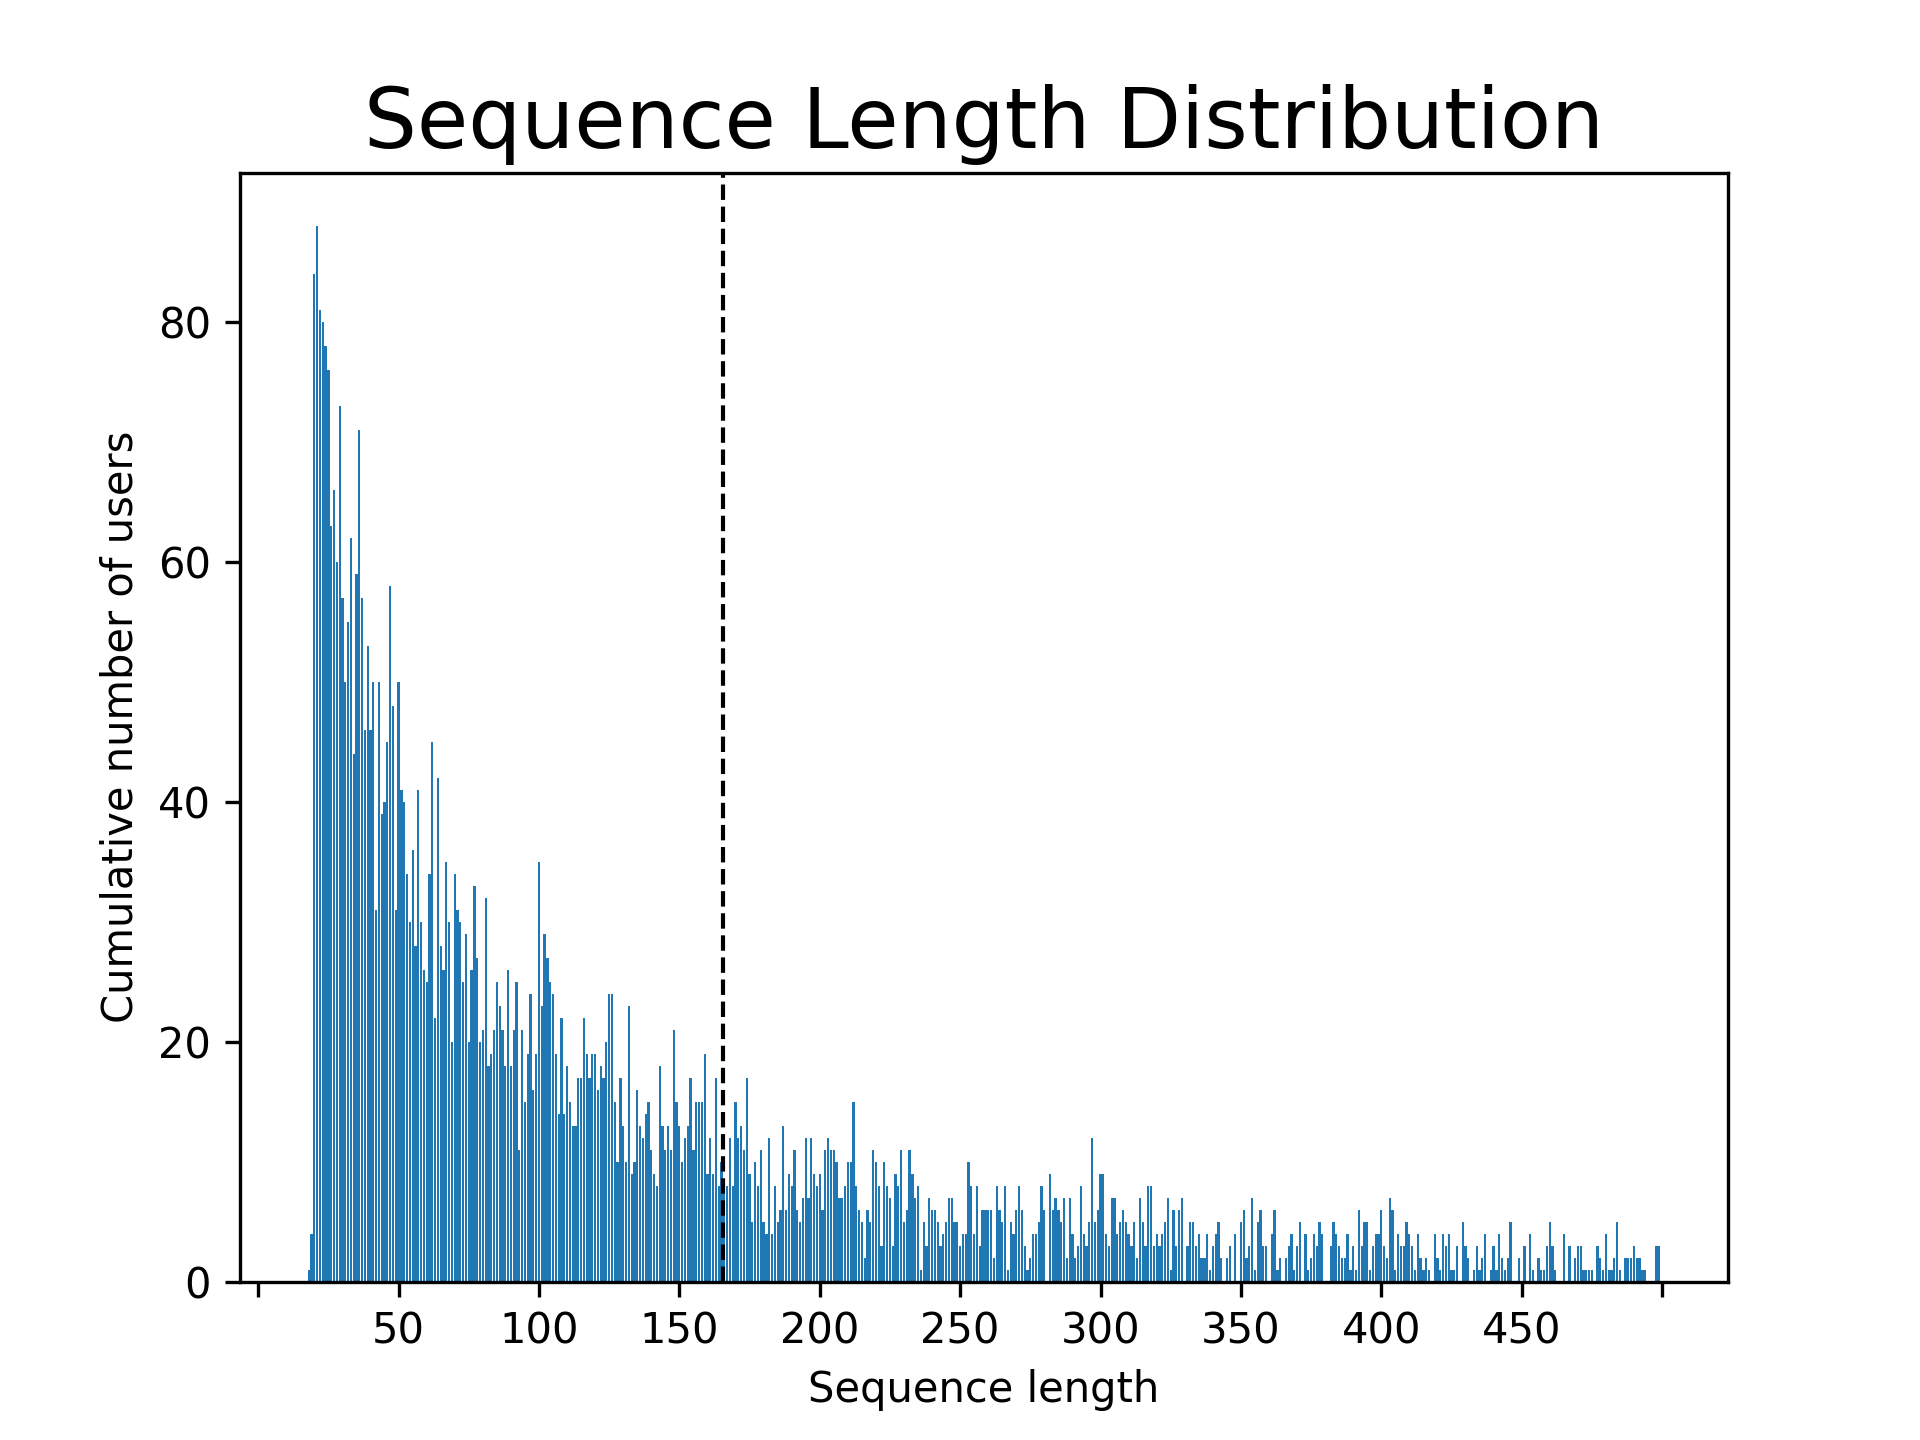
\includegraphics[width=0.5\columnwidth]{images/plots/seq_len_dist_ml.png}}
        \subfloat[Amazon Beauty]{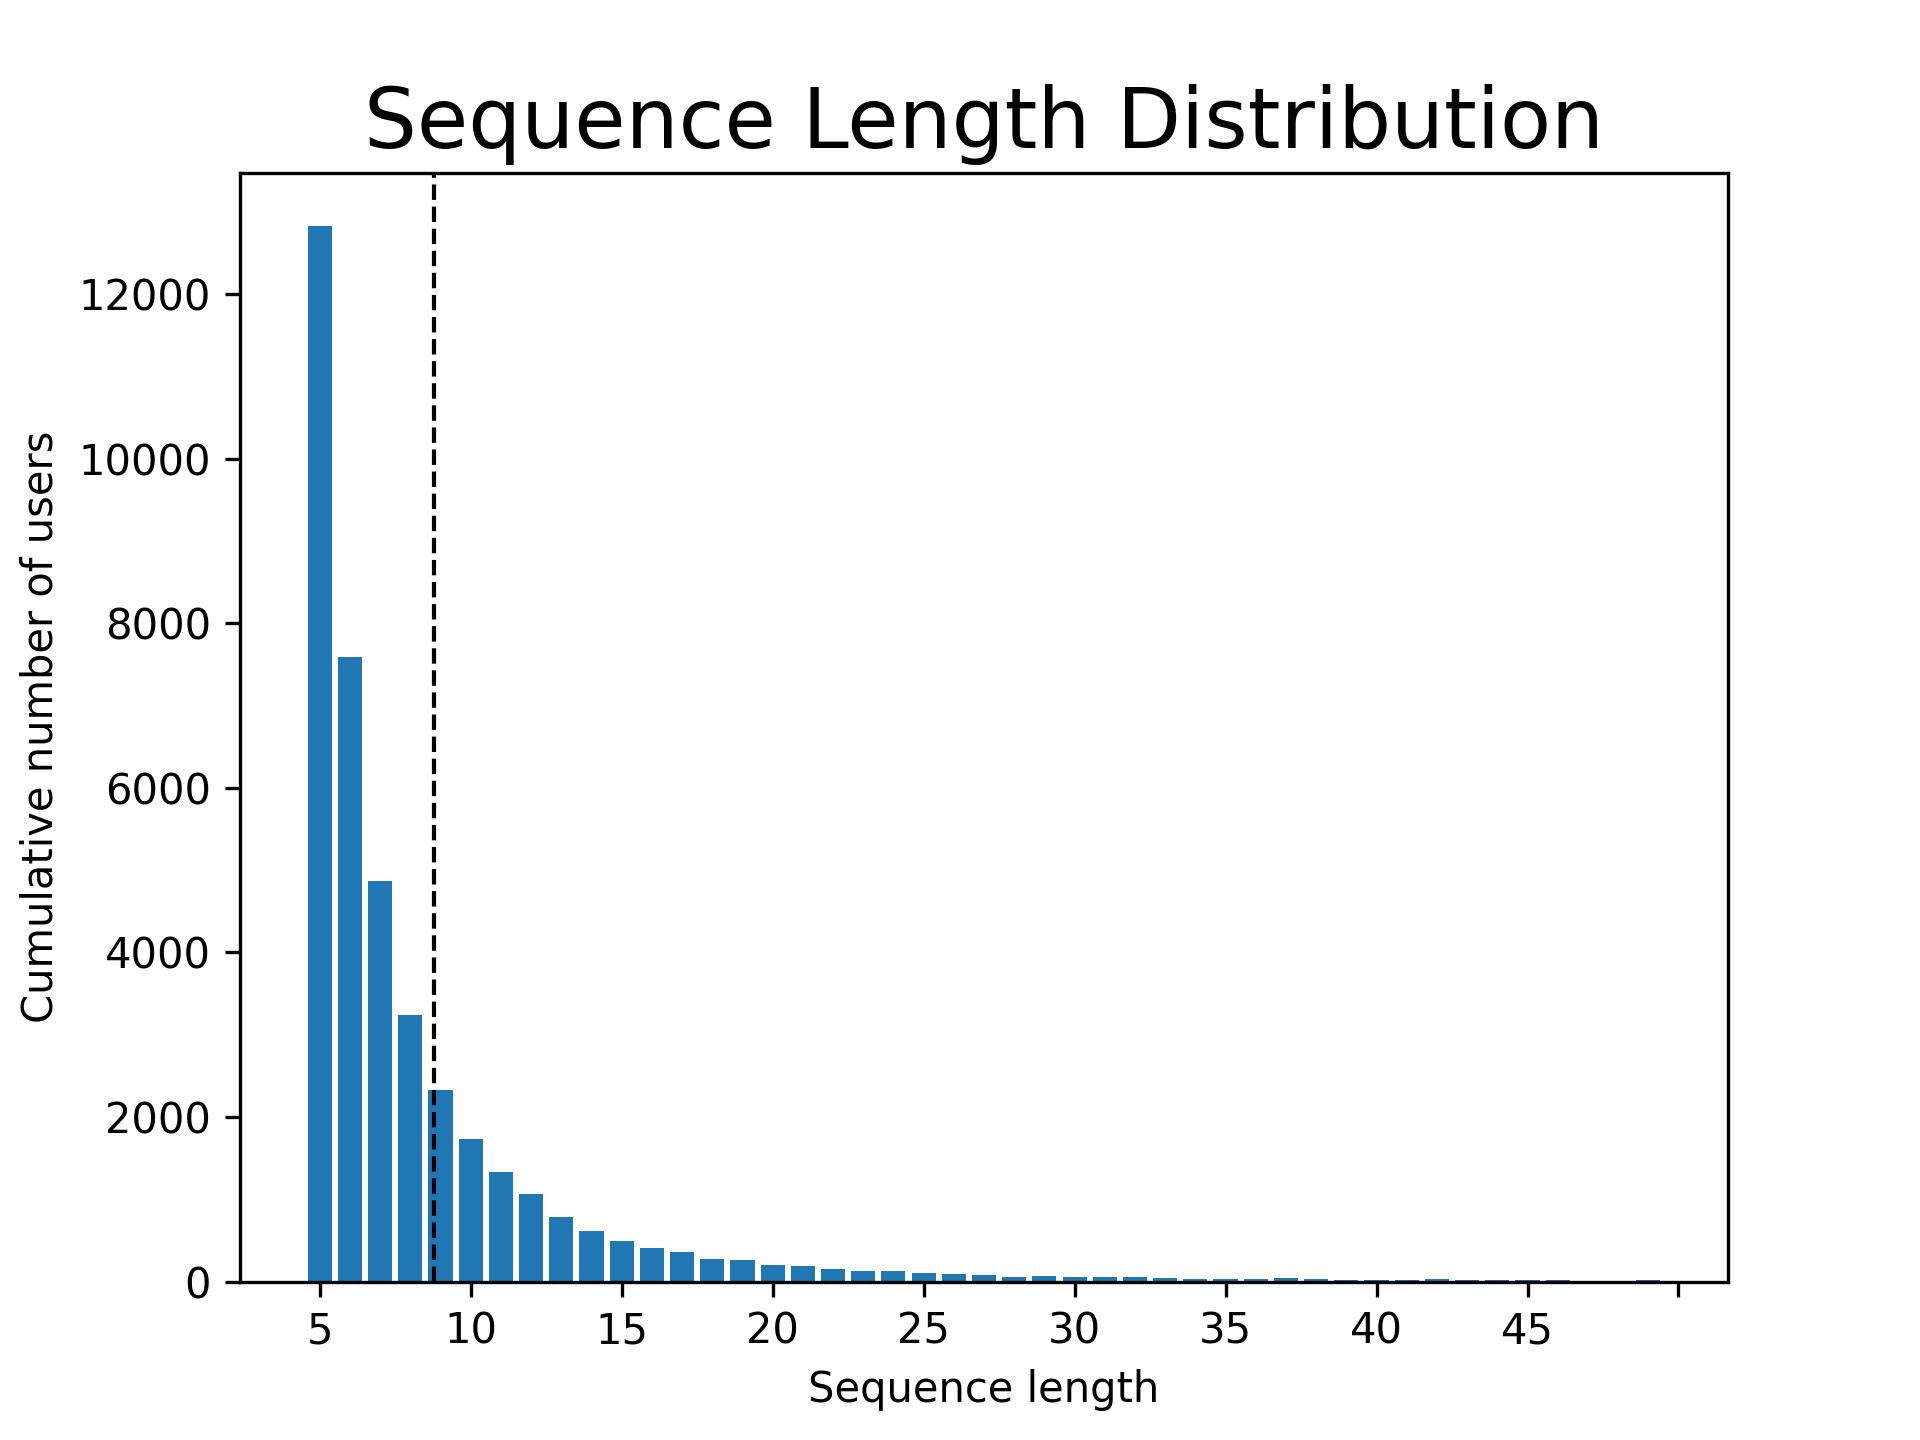
\includegraphics[width=0.5\columnwidth]{images/plots/seq_len_dist_beauty.png}}
    \caption{The sequence length distributions of our datasets}
    \label{fig:seq_len_dist}
\end{figure}

In our case, we have only one sequence of reviews per user, namely the list of all the reviews they left, ordered by time. The sequence length is thus the number of reviews given by each user. With a mean sequence length of 8.8, the Amazon Beauty dataset consists of short sequences. In contrast, the MovieLens 1M dataset has longer sequences with a mean length of 165.5 reviews per user. We picked the two datasets to make sure our system can make accurate predictions for long and short sequences. Additionally, the datasets include timestamps for every event. Timestamps give us a notion of time. We can gather information about sessions where users are active and idle.


\section{Data Partition}
\label{sec:data_partition}
Following the literature for sequential recommender systems, we split our dataset~\cite{kang2018self, sun2019bert4rec}. The last item in the sequence of every user will be the test set, the second to last item will be the validation set, and the rest of the items we use for training.

We have created an illustrative example of the split dataset for one user, shown in Figure~\ref{fig:datasplit}.

The aim is to have our final system predict for every user the last item in the sequence, the test set, as accurately as possible.

\begin{figure}[htbp]
\centering
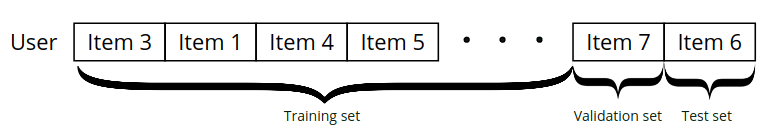
\includegraphics[width=0.8\textwidth]{images/illustrations/datasplit.png}
\caption{Example data partition for one user}
\label{fig:datasplit}
\end{figure}


\section{Evaluation Procedure}
\label{sec:test_procedure}
Let a negative item be an item that is not in the sequence of a user meaning the user has not engaged with the item yet. We now choose 100 random negative items that the user has not engaged with and
add the last item in the sequence (the test set item) (as is common in the literature~\cite{ying2018graph}). These 101 items get fed to the system for evaluation. The system will then output a probability for every item. Ideally, the test set item gets the highest probability, which would mean that the system made the correct prediction.

We follow the same procedure for every model that we evaluate to ensure that the results are comparable. It is worth noting that the literature is not very consistent when it comes to the evaluation of models. The number of negative items used for predictions may be higher or lower. A higher number of negative items will reduce the accuracy since it becomes more difficult to make a prediction, as the number of possible items increases. Consequently, we can not let the system output a prediction for every possible item given that every dataset has a different amount of total items. Hence we limit our predictions to 100 random negative items.


\section{Evaluation Metrics}\label{sec:metrics}
For our evaluation, we use the following standard metrics:

\begin{enumerate}
    \item \textbf{Hit Rate}
    
    \item \textbf{Normalized Discounted Cumulative Gain (NDCG)}
    
    \item \textbf{Mean Average Precision (MAP)} 
\end{enumerate}

A detailed explanation plus example calculation of the metrics can be found in Section~\ref{sec:standard_metrics}

% D.
% this sort of heavy teaching of what metrics are, that should get out of the way by putting it into the background
% in experimental setup, we should be moving on quickly before we bore our readers with lots of information they don't care and need. And we just refer to the detailed explanations in the background.
% Otherwise, the lengthy explanations break the rhythm and nobody wants to read on.
% 

% T.
% Ok gonna move it to background and cite here


\section{Training Setup}
\label{sec:training_setup}
Before the design and training of our hybrid sequential recommender system, we first have to implement, train, and evaluate our BERT model and our classic model. To get the most accurate prediction results, we have to make sure to follow good training practices.

\subsection{Overview of Implementations}

\paragraph{BERT Implementation}
Our primary model is based on BERT and an adaption of BERT4Rec's code basis~\cite{Githubbert4rec} (see Section~\ref{sec:bert_recommendations} for more details on BERT for recommendations). Although BERT was designed originally for NLP tasks, we can reuse most of the original BERT code maintained by Google~\cite{Githubbert} with only minor adaptions. Because learning the order of words in a sentence and learning the sequential order of interactions between a user and items are closely related tasks.  

% code upgrade
Since all of the code in BERT was written with TensorFlow version 1 we decided it is worthwhile to upgrade the code to TensorFlow version 2. The new version of TensorFlow comes with many valuable improvements~\cite{Tensorflow}. In the old TensorFlow version, the user had to manually build a syntax graph, add variables to it, compile it and then pass it to a session. This process can be tedious and strenuous to debug. By default TensorFlow 2.x supports eager execution, which means we can evaluate operations directly, and syntax graphs and sessions are no longer needed. The upgrade increases the code execution speed and reduces the training time. Additionally, many of the previously scattered high-level APIs have been grouped into one library called Keras.

\paragraph{Model-based Implementation}
Our implementation of the classic model is in part based on a codebase that implements various state-of-the-art sequential recommender systems~\cite{seqrecsota}. We unified input, output as well as evaluation of the model. All of this is done to ensure we can hybridize all our models easily. 

% D.
% I'm thinking all this presentation/selling of the code is too heavy and too important to be sold just on the side. Could belong in the system design. Not sure because not a "design" thing either. Maybe fine here.
% 

% D.
% What about the implementation of Caser? I might have missed sth. but I thought we do Caser too and the fact that it's one of the three headers in the related work chapter indicated so. Thought we had three systems, not just two. At least that's what I remember from the proposal but from what I can see in the tex structure I guess we're now down to two, Markov chains and Bert. 
%
% T.
% It is still part of the code base and fully functional. I just removed it from the thesis because I think it would take too much time and space to understand and present the model. I put my focus on the other two models (in the thesis). 
% 
% D.
% ok, fine


\subsection{Configuration of the Implementations}
\paragraph{Adam Optimizer}
The choice of optimizer can affect not only the training time but also the accuracy of a model. A traditional stochastic gradient descent performs updates in regular steps and does not take into account preceding gradients. If we picture a ball rolling down a slope, it accelerates and picks up momentum over time. That is the basic idea behind momentum optimizers. When updating the weights, we factor in a momentum vector to accelerate the gradient calculation~\cite{geron2019hands}. One of the most popular momentum optimizers with nearly 80k citations in the literature is Adam and stands for adaptive estimates of moments~\cite{kingma2014adam}. The algorithm for Adam is defined as follows:

\begin{equation}
\setlength{\jot}{19pt}
    \begin{aligned}
        m_t&\leftarrow \beta_1*m_{t-1}+(1-\beta_1)*g_t  \\
        v_t&\leftarrow\beta_2*v_{t-1}+(1-\beta_2)*g_t^2 \\
        \hat{m_t}&\leftarrow\frac{m_t}{1-\beta_1^t} \\
        \hat{v_t}&\leftarrow\frac{v_t}{1-\beta_2^t} \\
        \theta_t&\leftarrow\theta_{t-1}-\eta\frac{\hat{m_t}}{\sqrt{\hat{v_t}}+\epsilon} 
    \end{aligned}
    \label{equation:Adam}
\end{equation}

In the algorithm sketched in Equation~\ref{equation:Adam}, $g_t=\Delta_{\theta}f_t(\theta)$ is the gradient at time $t$. It is the partial derivative of function $f_t$ with parameter $\theta$. $m_t$ is the exponential moving average of the gradient and functions as the first moment estimate (or mean). $v_t$ is the exponential moving average of the squared gradient. It is the second raw moment estimate (or uncentered variance). The bias terms $b_1,b_2\in [0,1)$ regulate the exponential decay. Since the moving averages are biased towards zero, in the beginning, we calculate the bias-corrected terms $\hat{m_t}$ and $\hat{v_t}$. In the last step of the Adam algorithm, our learning rate $\eta$ controls how much we change the model weights after each training step.

\paragraph{Training the models}
For the optimizer, we use Adam with the bias terms $\beta_1=0.9$ and $\beta_1=0.999$ for the exponential decay of the moving averages. That corresponds to the default value in TensorFlow. 

\begin{figure}[htbp]
    \centering
        \subfloat{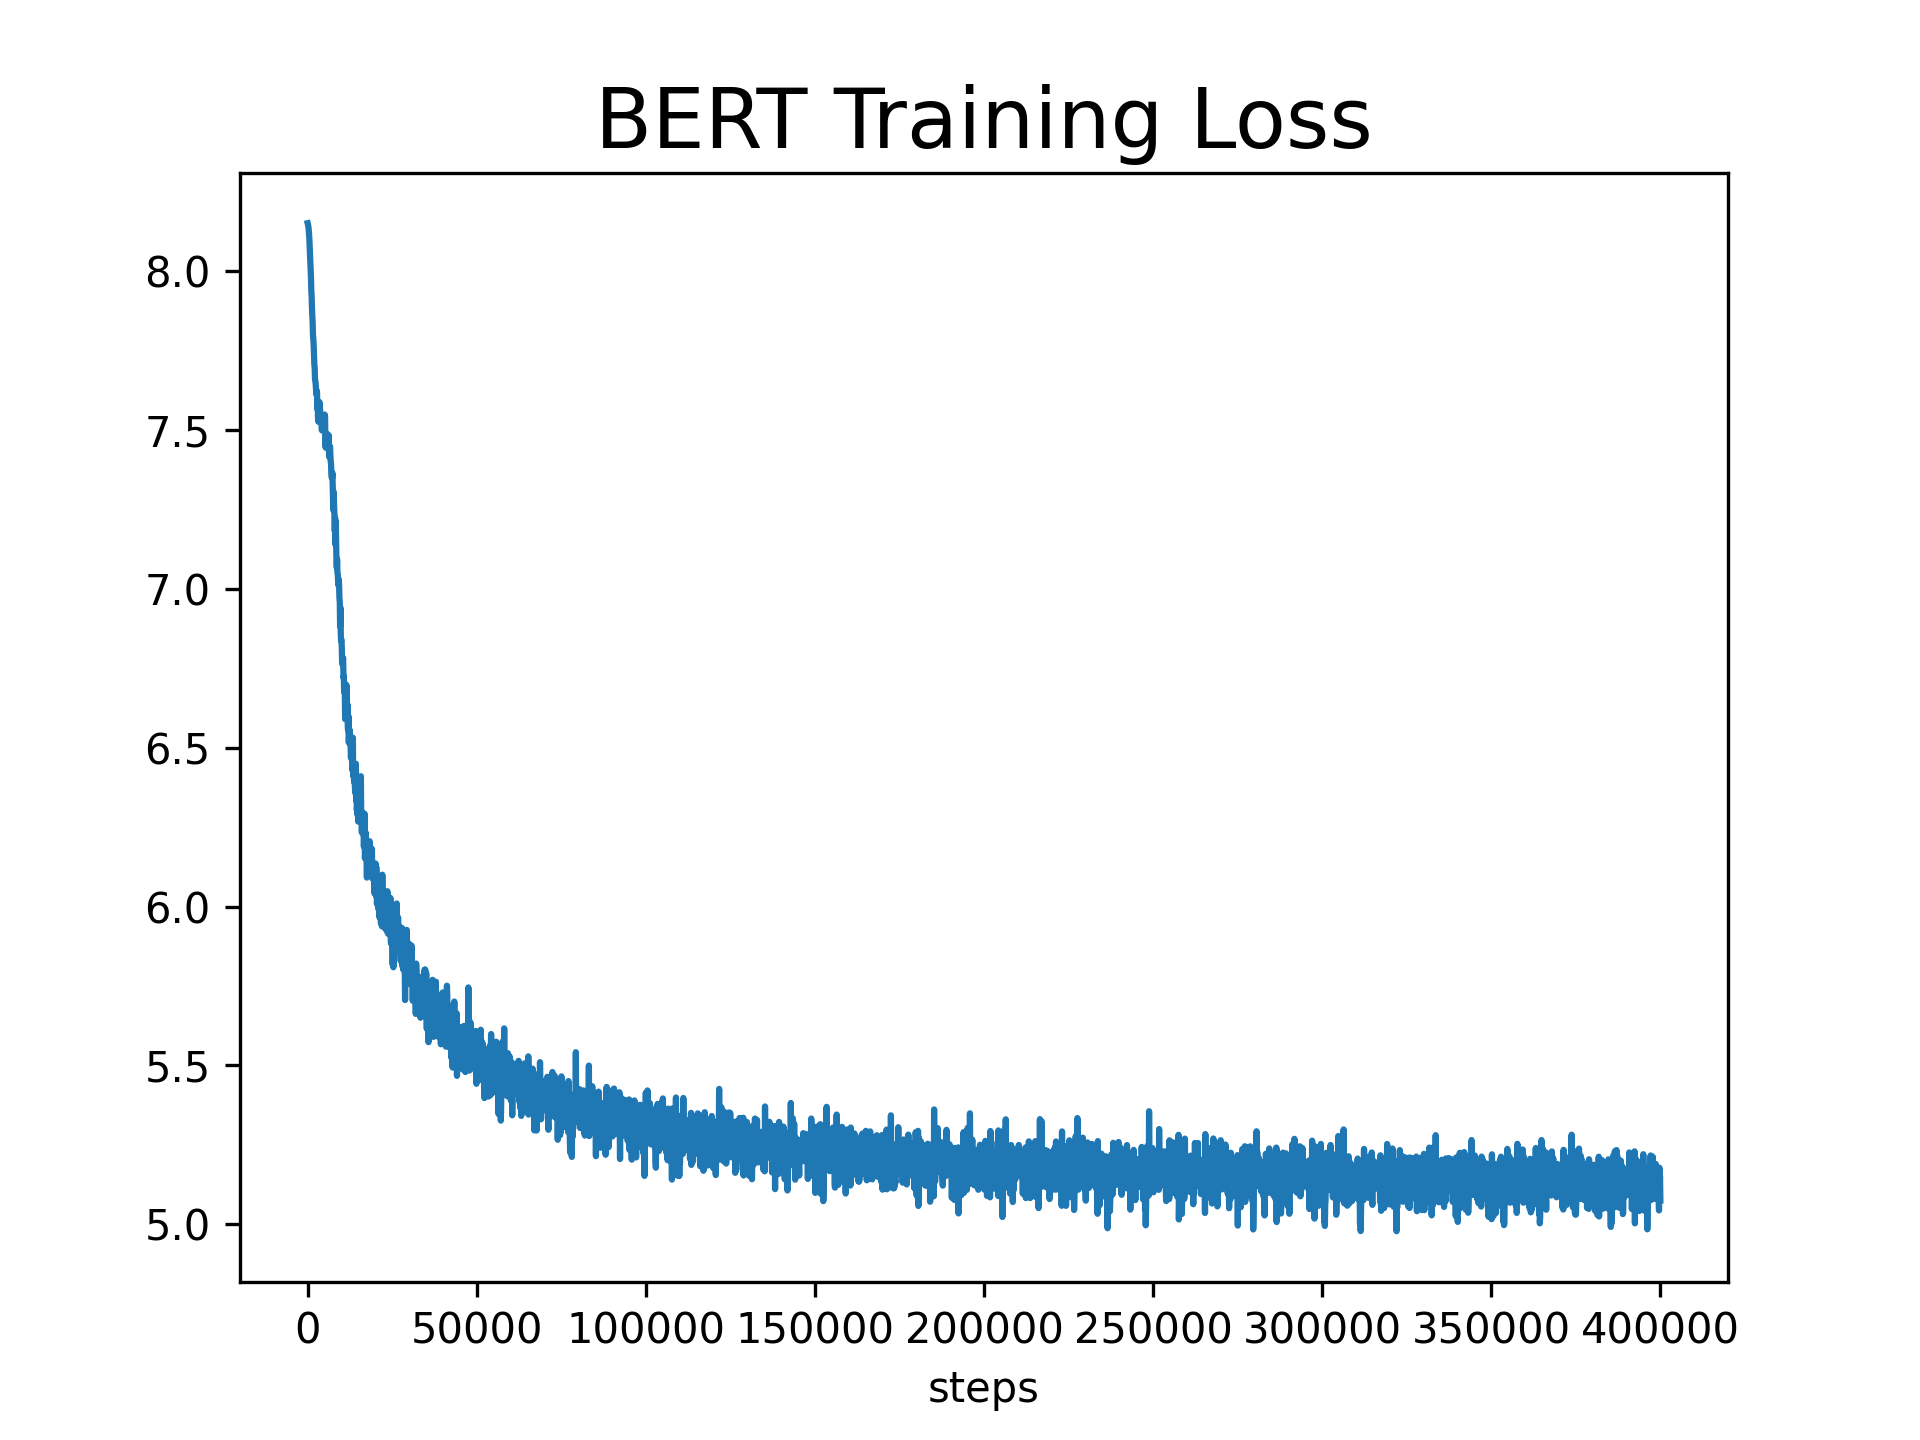
\includegraphics[width=0.5\columnwidth]{images/plots/bert_training_loss.png}}
        \subfloat{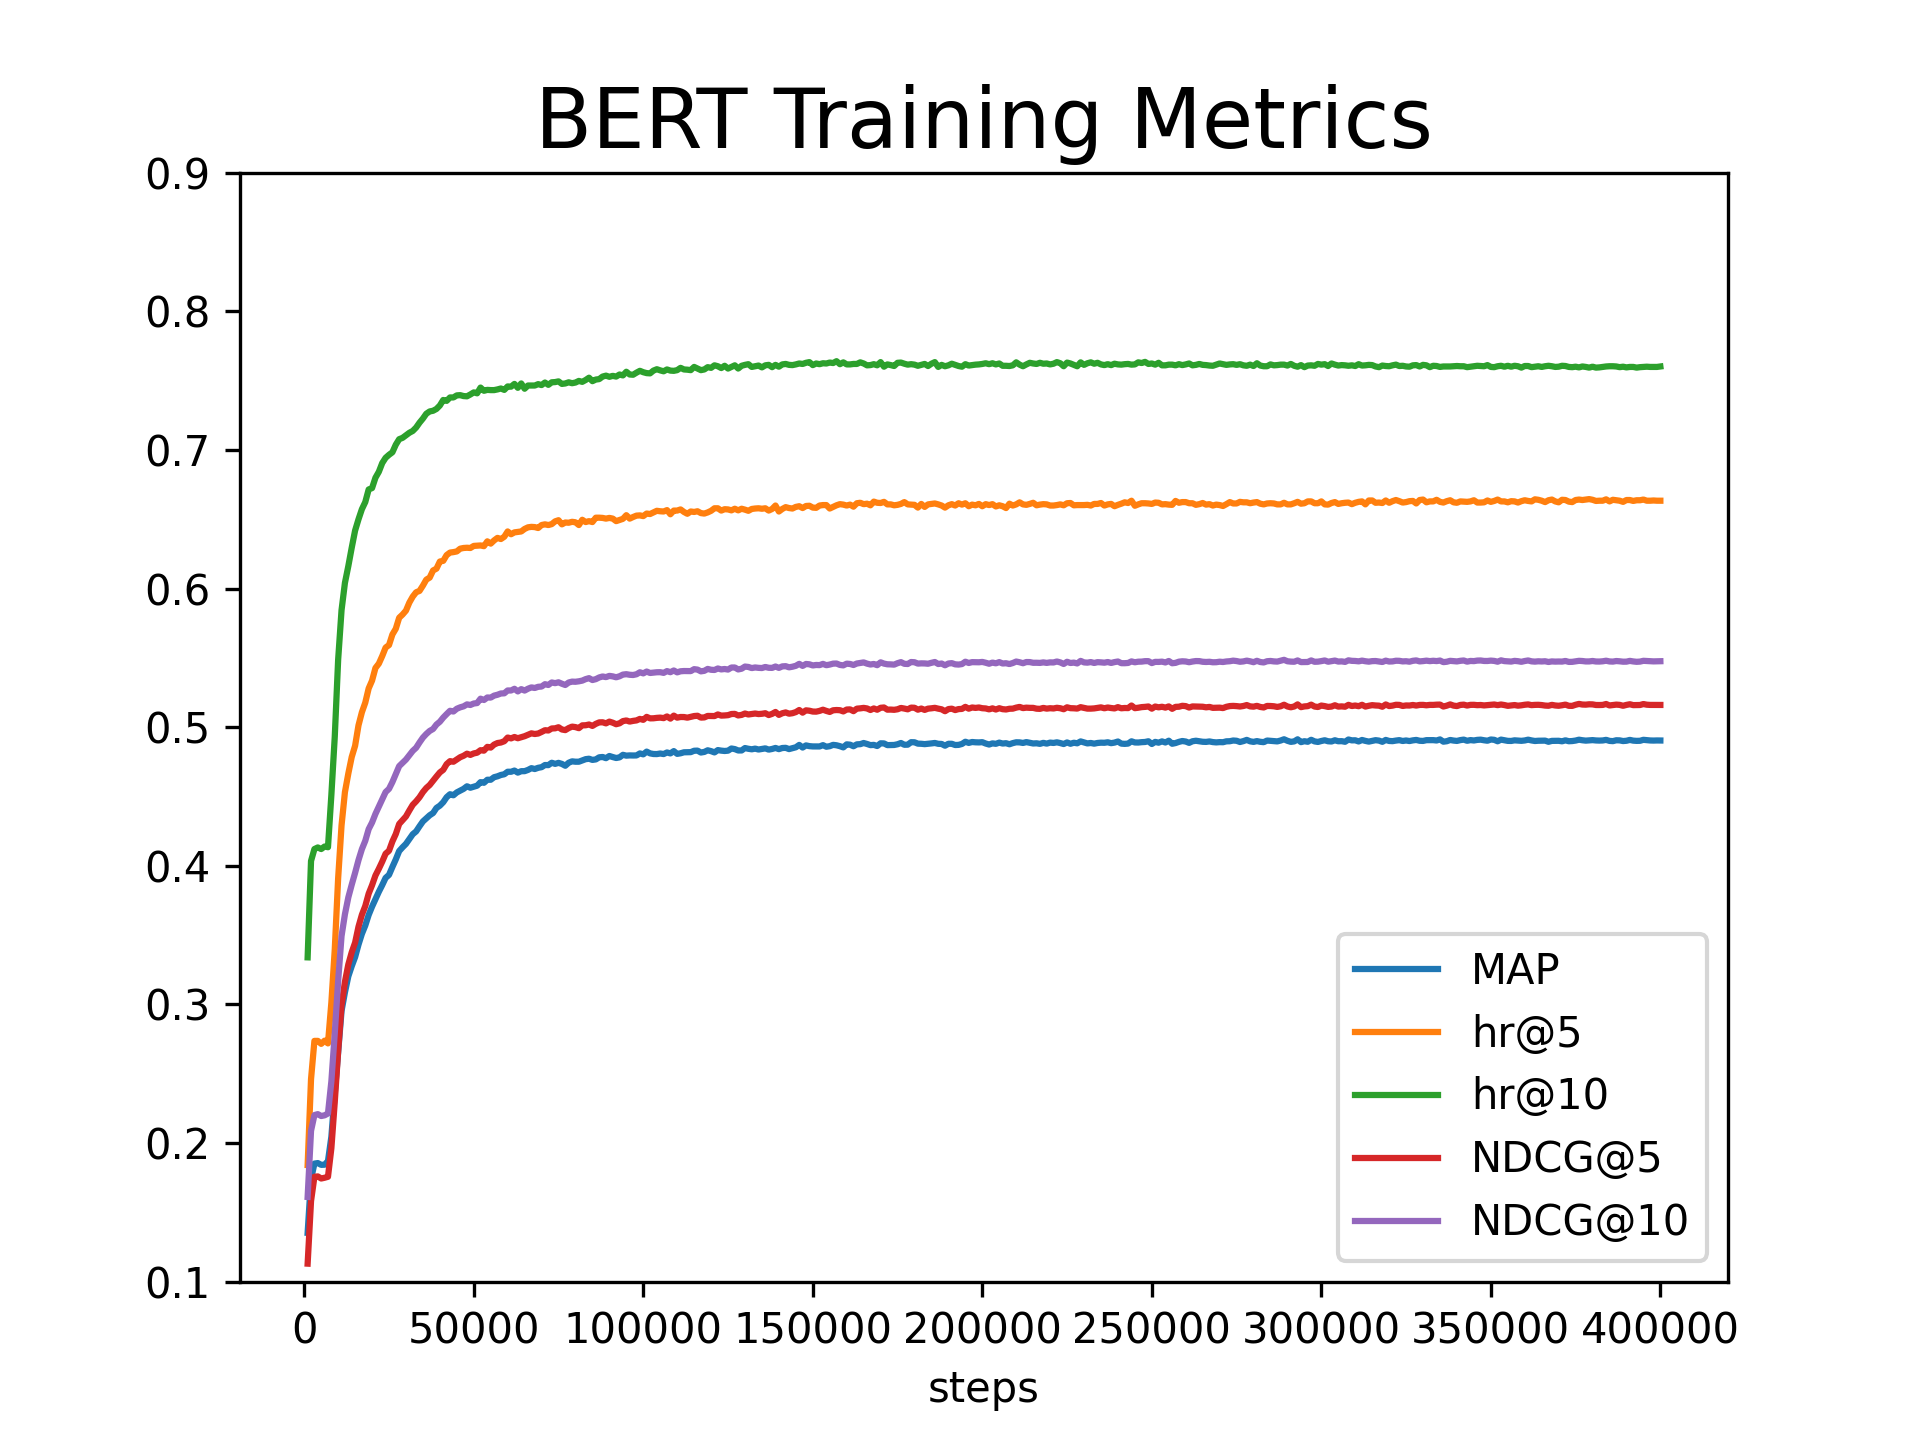
\includegraphics[width=0.5\columnwidth]{images/plots/bert_train_metrics.png}}
    \caption{BERT4 training metrics and training loss for the MovieLens 1M dataset}
    \label{fig:BERT_training}
\end{figure}

In Figure~\ref{fig:BERT_training}, we have plotted the training loss of BERT over time for the MovieLens 1M dataset. It is an indicator of how well the model has learned the training data. Each training step represents one training iteration with one batch of data. We use a batch size of 256 sequences from users.

\paragraph{Overfitting}
To make the evaluation fair, we try to follow the same principles for all models when training. As described in the Section \nameref{sec:data_partition}, we have split our data into training, validation, and test set. The validation set is used during training to evaluate and optimize the different hyperparameters. It is generally good practice to optimize hyperparameters using a separate validation set and not on the test set. Otherwise, we may risk that the model works well on our test set but not for new data. Similarly, finding the optimal training time is not a trivial task. If we train too little the model will have poor accuracy. But more training is only beneficial up to a particular point. As we train, we aim to minimize the loss function. In Figure~\ref{fig:BERT_training}, we can see that the training loss decreases over time, and the accuracy of predictions for the MovieLens 1M dataset increases at each training step. However, at some point, we may risk that our loss function fits the training data too closely. This phenomenon is called overfitting~\cite{hawkins2004problem}. Although a model that overfits has learned the training data well, it may not make accurate predictions for novel data it has not seen yet.

\begin{figure}[htbp]
    \centering
        \subfloat{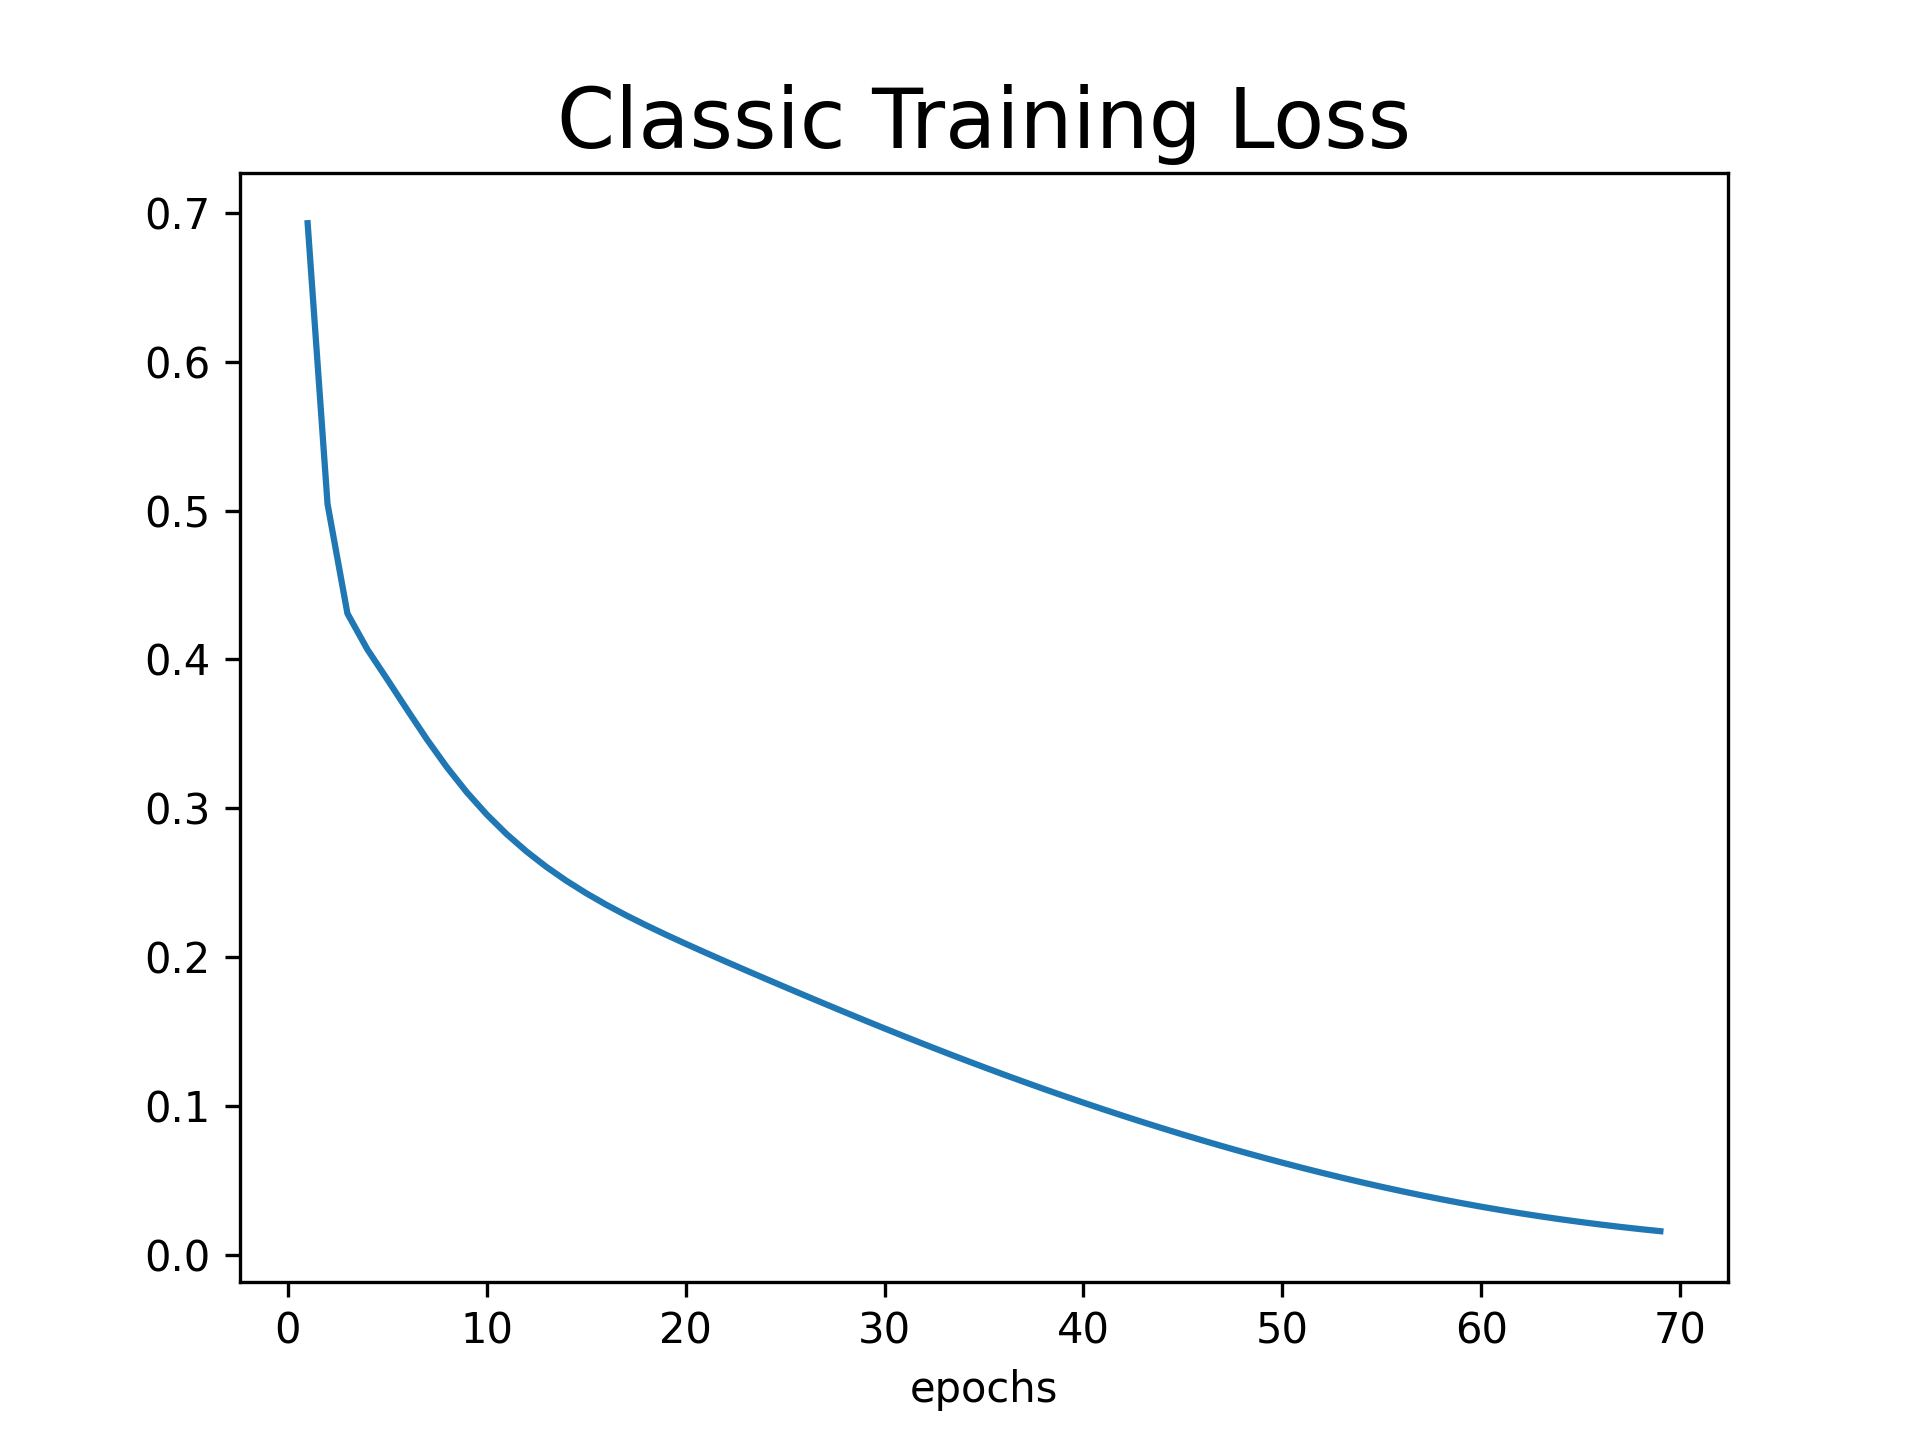
\includegraphics[width=0.5\columnwidth]{images/plots/classic_train_loss.png}}
        \subfloat{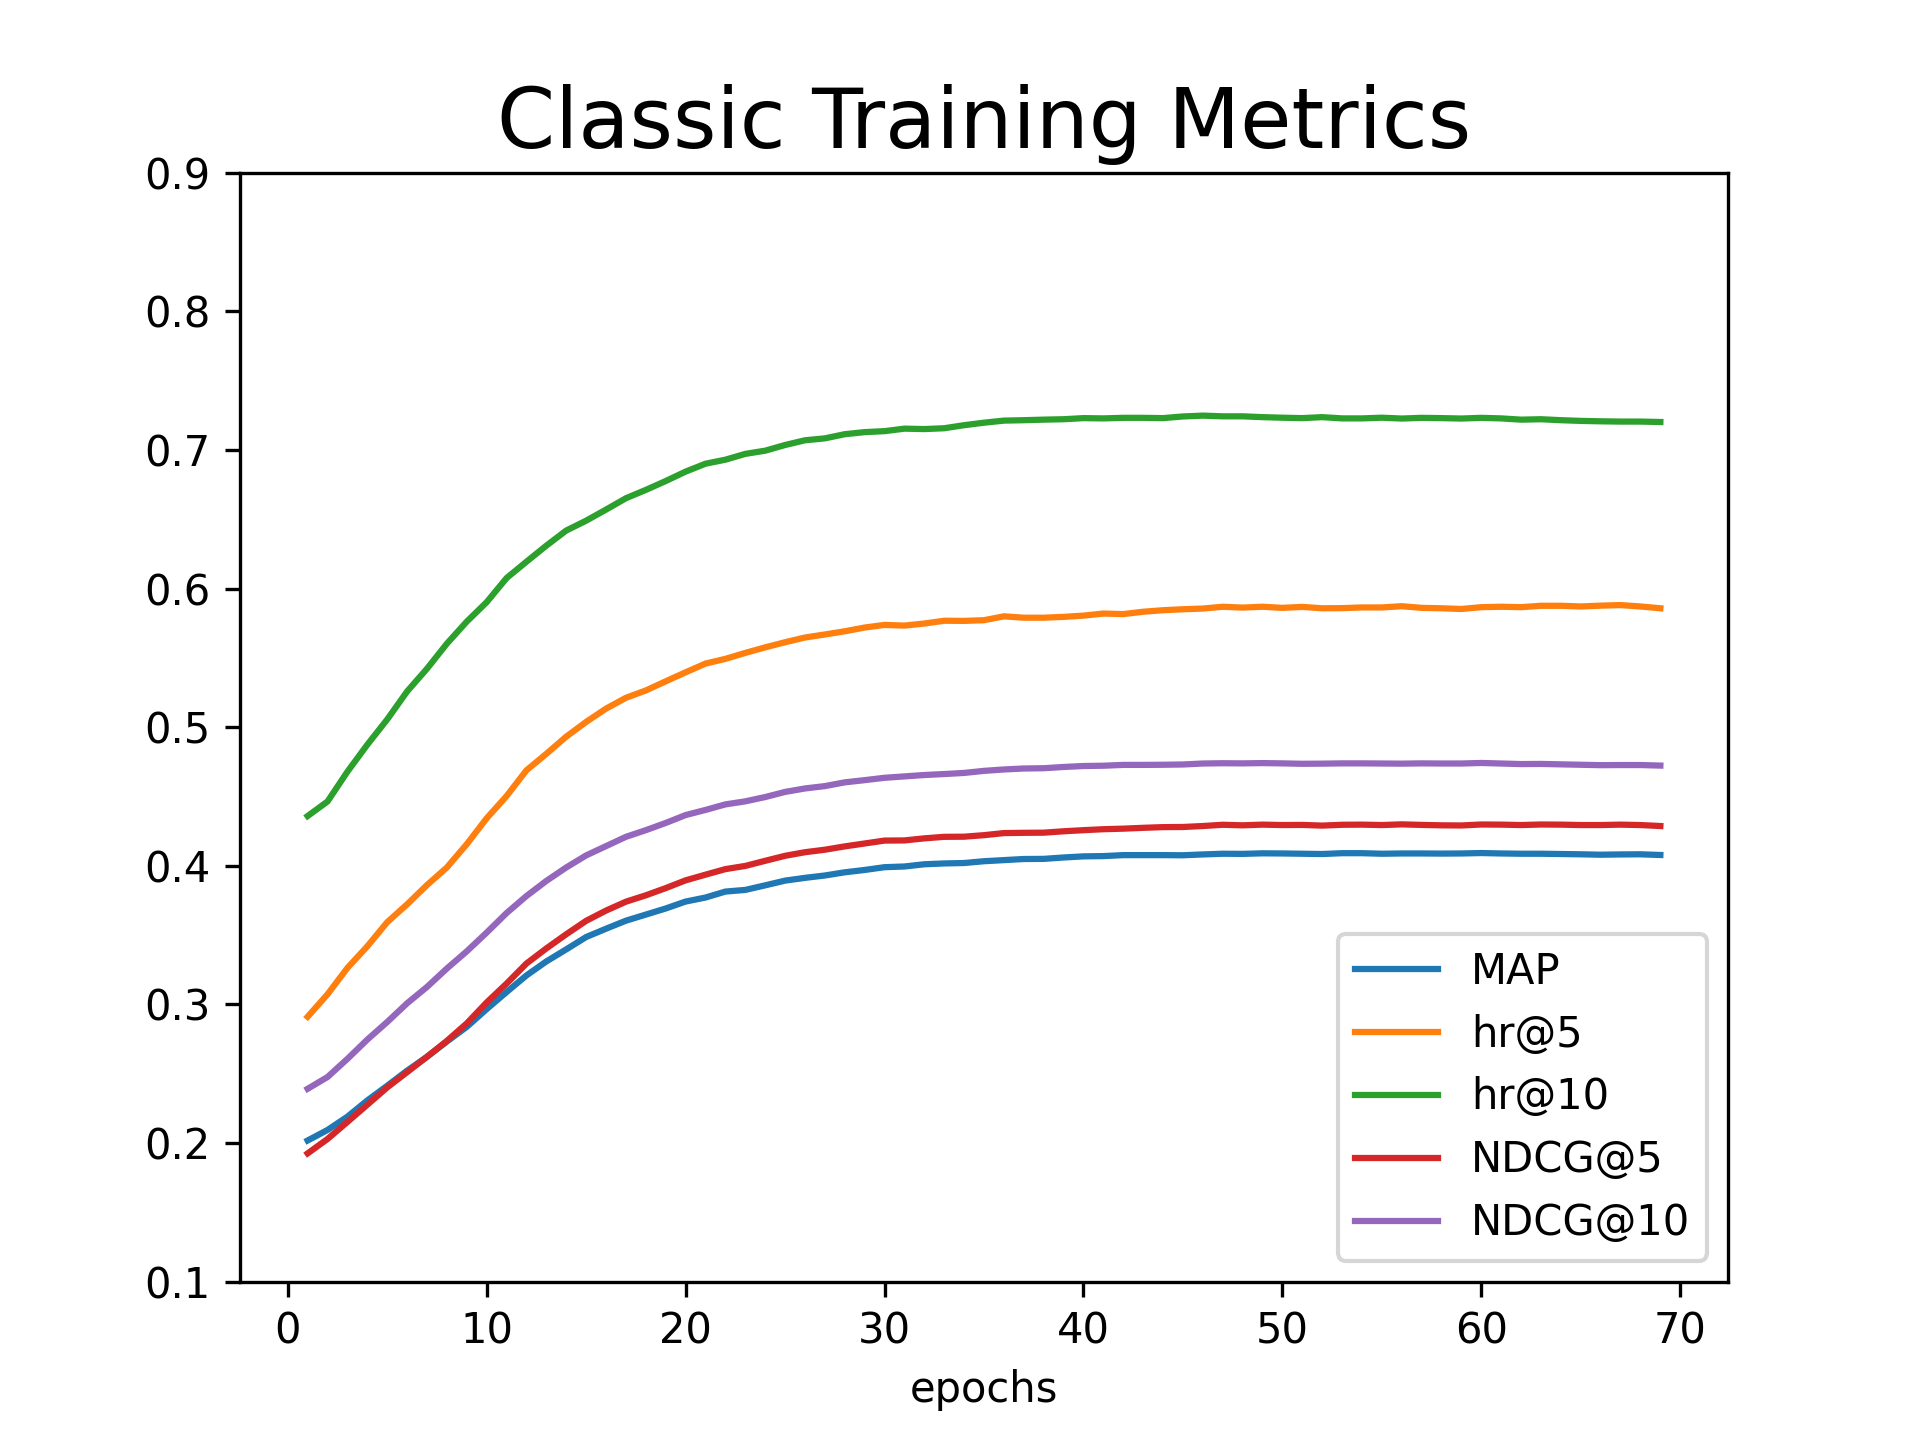
\includegraphics[width=0.5\columnwidth]{images/plots/classic_train_metrics.png}}
    \caption{Classic training metrics and training loss for the MovieLens 1M dataset}
    \label{fig:classic_training}
\end{figure}

\paragraph{Early Stopping}
To prevent overfitting, we have to implement some form of early stopping. We experiment with different training steps and stop training BERT after 400000 steps. For our classic model, we save the model weights during training. That way, we can later restore the model with the optimal hyperparameters. One epoch represents one iteration through the whole training dataset. After every epoch, we evaluate the model with the validation set by adding up all the evaluation metrics. Figure~\ref{fig:classic_training} shows the evaluation of the validation set over time for our classic model and the MovieLens 1M dataset. We implement early stopping and stop training when the accuracy does not improve for 20 epochs. The final model is the model that had the best predictions of the validation set.

\paragraph{Learning Rate}
We optimize the learning rate via manual tuning i.e., with a grid search. We experiment with different learning rates and find that a learning rate of $1e^{-3}$ yields results that are not accurate enough. A learning rate of $1e^{-5}$ increases the training time significantly without an accuracy improvement. We settle for a learning rate of $1e^{-4}$. A plot of the training loss over time for our classic model is depicted in Figure~\ref{fig:classic_training}.

% D.
% I like the point-by-point review of the design aspects of the neural architecture

\subsection{Infrastructure}
For training and evaluation, we use Google Colab Pro. The servers run Ubuntu 18.04 LTS (Bionic Beaver) and feature a Tesla P100-PCIE-16GB GPU, six Intel(R) Xeon(R) CPUs @ 2.20GHz and 27 GB of RAM. 